\documentclass[11pt]{report}
%
%2345678901234567890123456789012345678901234567890123456789012345678901234567890
%        1         2         3         4         5         6         7         8
%
% $Id: main.tex,v 1.2 2002-03-11 11:45:33 jabril Exp $
%
\usepackage[a4paper,offset={0pt,0pt},hmargin={2cm,2cm},vmargin={1cm,1cm}]{geometry}
\usepackage[catalan]{babel}
\usepackage{graphics}
\usepackage[dvips]{graphicx}
%% pstricks
\usepackage[dvips]{pstcol}
\usepackage{pstricks}
%\usepackage{pst-node}
%\usepackage{pst-char}
%\usepackage{pst-grad}
%% bibliography
\usepackage{natbib}
%% latex2html
\usepackage{url}
\usepackage{html}     
\usepackage{htmllist} 
%% tables    
\usepackage{dcolumn}
%\usepackage{colortbl}
%\usepackage{multirow}
%\usepackage{hhline}
%\usepackage{tabularx}
%% seminar
%\usepackage{semcolor,semlayer,semrot,semhelv,sem-page,slidesec}
%% draft watermark
%\usepackage[all,dvips]{draftcopy}
%\draftcopySetGrey{0.9}
%\draftcopyName{CONFIDENTIAL}{100}
%% layout
\usepackage{fancyhdr} % Do not use \usepackage{fancybox} -> TOCs disappear
%\usepackage{lscape}
%\usepackage{rotating}
%\usepackage{multicol}
\usepackage{verbatim}
%\usepackage{version}
%% fonts
\usepackage{times}\fontfamily{ptm}\selectfont
\usepackage{t1enc}

\input ColorDefs.tex %%%%% Colors for gff2ps
\input defs.tex      %%%%% Common Definitions File

%%%%% Setting text for footers and headers
\fancyhead{} % clear all fields
\fancyfoot{} % clear all fields
\fancyhead[RO,LE]{\thepage}
\fancyhead[LO,RE]{\shorttit\quad\rightmark}
\fancyfoot[LO,LE]{\small\textbf{\genomelab}}
\fancyfoot[CO,CE]{\small\textsl{\authorshort}}
\fancyfoot[RO,RE]{\small\textbf{\today}}
\renewcommand{\headrulewidth}{1pt}
\renewcommand{\footrulewidth}{1pt}
%%%%%

\begin{document}

%
% $Id: title.tex,v 1.4 2002-03-13 10:14:20 jabril Exp $
%
%2345678901234567890123456789012345678901234567890123456789012345678901234567890
%        1         2         3         4         5         6         7         8
%
\pagestyle{empty}

\begin{titlepage}

\ \vfill
\begin{center}
\textbf{\Huge \tit} \\[5ex]
\authorslist      \ \\[5ex]

\textbf{\large --- \today ---} \\[10ex]

\vfill

\begin{raggedleft}
\showaffiliation
\showemails
\end{raggedleft}
\end{center}

\end{titlepage} %'

\ \vfill
\versioncontrol

\newpage

\begin{abstract}
\begin{center}
\parbox{0.75\linewidth}{
\progdesc
} % parbox
\end{center}
\end{abstract}

\newpage

\ \vfill
\begin{flushright}
\begin{minipage}[c]{30ex}
A la paci�ncia de les dones,\\ en especial de la meva\ldots \verb+;^)+
\end{minipage}
\end{flushright}
\vfill

\newpage % EMPTY PAGE


\newpage %%%%%%%%%%%%%%%%%%%% FRONTMATTER

%
% $Id: tocs.tex,v 1.3 2002-03-13 10:14:20 jabril Exp $
%
%2345678901234567890123456789012345678901234567890123456789012345678901234567890
%        1         2         3         4         5         6         7         8
%
\pagenumbering{roman}
\setcounter{page}{1}
\pagestyle{fancy}
% Marks redefinition must go here because pagestyle 
% resets the values to the default ones.
\renewcommand{\sectionmark}[1]{\markboth{}{\thesection.\ #1}}
\renewcommand{\subsectionmark}[1]{\markboth{}{\thesubsection.\ \textsl{#1}}}

\tableofcontents \addcontentsline{toc}{chapter}{�ndex}

\listoftables    \addcontentsline{toc}{section}{�ndex de Taules}

\listoffigures   \addcontentsline{toc}{section}{�ndex de Figures}


\newpage %%%%%%%%%%%%%%%%%%%% MAINMATTER
\pagenumbering{arabic}
\setcounter{page}{1}

%
% $Id: intro.tex,v 1.2 2002-03-13 10:14:10 jabril Exp $
%
%2345678901234567890123456789012345678901234567890123456789012345678901234567890
%        1         2         3         4         5         6         7         8
%
\chap{Introducci�}

\sctn{Aspectes Biol�gics.}

\subsctn{Les seq��ncies gen�miques.}

Entre finals del 1989 i principis del 1990 es van definir les bases del que m�s tard s'anomenaria el Projecte Genoma Hum�, que consistiria en obtenir la seq��ncia de nucle�tids que composa les mol�cules de DNA de la nostra esp�cie.
Gr�cies a les noves tecnologies, en especial de les m�quines seq�enciadores autom�tiques i del m�tode de seq�enciaci� per \textit{shotgunn}, en els darrers anys hem pogut assistir a l'explossi� ... de les dades gen�miques sobre seq��cies de diferents esp�cies (veieu la taula~\ref{tbl:seqdgenomes}).

\begin{table}[!b] %%%%%%%%%%%%%%%%%%%%%%%%%%%%%%
\begin{center}
\cpt{tbl:seqdgenomes}
    {Fites en la seq�enciaci� de genomes.}
    {Es resumeixen aqu� les fites m�s importants en la seq�enciaci� de genomes. Cal destacar l'increment en la mida dels genomes que s'han pogut analitzar. En el cas del genoma hum�, actualment es disposa d'un primer esborrany que es correspon amb les dades publicades el febrer de l'any 2001, per� la seq�enciaci� encara continua i el ensamblatge definitiu encara trigar� un o dos anys m�s. El que anirem veient ser� el degoteig de cromosomes humans per als quals s'hagi aconseguit completar totes les etapes de la seq�enciaci�, com �s el cas dels cromosomes 20, 21 i 22.}
%
\input ./tables/seqdgenomes
%
\end{center}
\end{table}       %%%%%%%%%%%%%%%%%%%%%%%%%%%%%%


\subsctn{Homologia entre esp�cies.}


\begin{figure}[!t]
\begin{center}
\begin{minipage}[b]{0.5\linewidth}
\fbox{
 \includegraphics[trim= 25 100 25,clip,width=\linewidth]{./psfigures/GF004.ps}
} % fbox
\end{minipage}
\hspace{0.25cm}
\begin{minipage}[b]{0.45\linewidth}
\cpt{fig:homology4spec}
    {An�lisi de l'estructura g�nica mitjan�ant la homologia entre esp�cies.}
    {Esp�cies relativament properes no tan sols conserven, a nivell de seq��ncia, les regions codificants i la homologia sovint s'est�n m�s enll� dels senyals que delimiten els exons, els \textit{splice sites} o llocs d'\textit{splicing}. Aix� es pot apreciar en els dos alineaments de seq��ncies entre dues esp�cies molt pr�ximes com s�n la rata (\textit{Rattus norvegiques}) i el ratol� (\textit{Mus musculus}) de la regi� que cont� el gen de la hormona del creixement i els seus ort�legs corresponents. Si es fa el mateix comparant la seq��ncia en humans amb la del ratol�, encara que hi ha variaci� a nivell de les longituts dels introns, podem observar un patr� similar al del cas anterior. A mesura que ens anem allunyant en l'escala filogen�tica, la conservaci� de les regions intr�niques va desapareixent, com es pot comprovar per en els dos alineaments entre la regi� gen�mica de l'hormona del creixement en humans envers la regi� hom�loga en pollastre (\textit{Gallus gallus}) i el peix globus (\textit{Fugu rubripes}).}
\end{minipage}
\end{center}
\end{figure}


\sctn{Predicci� Computacional de Gens.}

\subsctn{De la seq��ncia de DNA a l'estructura de la prote�na.}

\begin{figure}[!t]
\begin{center}
\begin{minipage}[t]{0.5\linewidth}
\fbox{
 \begin{minipage}[c][5cm][c]{\linewidth}\hfill\end{minipage}
% \includegraphics[width=0.45\linewidth]{./psfigures/.ps}
} % fbox
\end{minipage}
\hspace{0.25cm}
\begin{minipage}[t]{0.45\linewidth}
\cpt{fig:sequencesignals}
    {Recerca computacional d'estructures g�niques en seq��ncies de DNA.}
    {...}
\end{minipage}
\end{center}
\end{figure}
 
\subsctn{Predicci� d'estructures g�niques basada en la homologia.}

\begin{figure}[!t]
\begin{center}
\begin{minipage}[t]{0.5\linewidth}
\fbox{
 \includegraphics[width=0.85\linewidth, trim= 10 10 20 10, clip]
                 {./psfigures/algo2.ps}
} % fbox
\end{minipage}
\hspace{0.25cm}
\begin{minipage}[t]{0.45\linewidth}
\cpt{fig:homologygenepred}
    {Predicci� d'estructures g�niques basada en la homologia.}
    {...}
\end{minipage}
\end{center}
\end{figure}


\subsctn{Reanotaci� de Genomes.}






%
% $Id: matimet.tex,v 1.2 2002-03-13 10:14:20 jabril Exp $
%
%2345678901234567890123456789012345678901234567890123456789012345678901234567890
%        1         2         3         4         5         6         7         8
%
\chap{Material i M�todes}

\sctn{Predicci� Computacional de Gens}

\subsctn{{\gnid}}

\begin{figure}[!t]
\begin{center}
\begin{minipage}[t]{0.5\linewidth}
\fbox{
 \includegraphics[width=0.45\linewidth]{./psfigures/geneid_flowchart.ps}
} % fbox
\end{minipage}
\hspace{0.25cm}
\begin{minipage}[t]{0.45\linewidth}
\cpt{fig:geneidflowchart}
    {Diagrama de la estructura interna del {\gnid}.}
    {Estructura interna del programa de predicci� computacional de gens {\gnid}... }
\end{minipage}
\end{center}
\end{figure}



\sctn{Analitzant la homologia entre humans i ratolins}


\begin{figure}[!t]
\begin{center}
\begin{minipage}[t]{0.5\linewidth}
\fbox{
\begin{minipage}[c][5cm][c]{\linewidth}\hfill\end{minipage}
% \includegraphics[width=0.45\linewidth]{./psfigures/.ps}
} % fbox
\end{minipage}
\hspace{0.25cm}
\begin{minipage}[t]{0.45\linewidth}
\cpt{fig:humushomology}
    {Analitzant la homologia entre humans i ratolins.}
    {...}
\end{minipage}
\end{center}
\end{figure}


\subsctn{{\sgp}}


\sctn{Protocol de reanotaci� del genoma hum�}


\begin{figure}[!t]
\begin{center}
\begin{minipage}[t]{0.5\linewidth}
\fbox{
\begin{minipage}[c][5cm][c]{\linewidth}\hfill\end{minipage}
% \includegraphics[width=0.45\linewidth]{./psfigures/.ps}
} % fbox
\end{minipage}
\hspace{0.25cm}
\begin{minipage}[t]{0.45\linewidth}
\cpt{fig:humgenreannot}
    {Diagrama del proc�s de reanotaci� del genoma hum� basat en la homologia amb ratol�.}
    {...}
\end{minipage}
\end{center}
\end{figure}

%
% $Id: results.tex,v 1.1 2002-03-11 11:44:55 jabril Exp $
%
\chap{An�lisi dels Resultats}
\sctn{}
\sctn{}
\sctn{}
\sctn{Automatitzaci� del proc�s de reanotaci� dels genomes}



\newpage %%%%%%%%%%%%%%%%%%%% BACKMATTER

\appendix

%%%%%%% BIBLIOGRAPHY
% 
\bibliographystyle{apalike}
% \bibliography{/home1/rguigo/docs/biblio/References}

\newpage %%%%%%%%%%%%%%%%%%%%%

\include{gfftools}

%
\end{document}
%
%%%%%%%%%%%%%%%%%%%%%%%%%%%%%%%%%%%%%%%%%%%%%%%%%%%%%%%%%%%%%%%%%%%%%%%%%%%%%%%%
